\documentclass[a4paper,11pt]{ltjsarticle}
\usepackage{amsmath, mathtools, mathbbol, amssymb, bm, fancyhdr, anyfontsize, subcaption, multirow, wrapfig, graphicx, hyperref, url, enumitem, ascmac, tikz, tikz-3dplot, makeidx}
\usetikzlibrary{arrows, angles, quotes}
\captionsetup{compatibility=false}

\hypersetup{
 pdfencoding=auto,
 setpagesize=false,
 bookmarksnumbered=true,
 bookmarksopen=true,
 colorlinks=true,
 linkcolor=blue,
 citecolor=blue,
 urlcolor=blue,
}

\makeindex
\numberwithin{equation}{section}
\usepackage[numbers]{natbib}
\usetikzlibrary{arrows, angles, quotes}
\renewcommand{\cite}[1]{\textsuperscript{\citep{#1}}}
\newcommand{\idx}[1]{#1\index{#1}}

\newcommand{\dlim}[2]{\displaystyle{\lim_{#1 \to #2}\:}}
\newcommand{\dint}[2]{\displaystyle{\int_{#1}^{#2}}}
\def\tick#1#2{\draw[thick] (#1)++(#2:0.12) --++ (#2-180:0.24)}
\def\N{100} % number of samples

\pagestyle{fancy}
\rhead{\textbf{\thepage}}
\cfoot{}
\renewcommand{\headrulewidth}{0pt}

\title{\textbf{統計計算の基礎}}
\author{Y-teraya}
\date{\today}

\begin{document}

\maketitle

\begin{abstract}
  本資料は,統計の基礎的な計算方法をまとめたものである.
  実験計画法を主として扱い,実務で直結する内容(Excel函数など)を備忘録として記しておく.
  ほか,線形代数や微分積分も取り扱う.

  また,総和$\sum$の記号に苦手意識を持っている人も多いので,理解して欲しい重要な式のみ$\sum$無しで表現した式も併記する.
\end{abstract}

\tableofcontents

\vspace{12pt}

\begin{center}
  \textbf{\color{blue}青文字}をクリックすると,対応したページに遷移します.
\end{center}

\clearpage

\section*{留意事項}

\begin{enumerate}
  \item 色付き文字やハイライトは重要事項または強調箇所である.
  \item 自身の好み(独断と偏見)で作成しているため,旧字体や座標を行列で記載している箇所がある.
  \item 本資料の著作権は,\href{https://creativecommons.org/licenses/by-nc-sa/4.0}{CC BY-NC-SA 4.0}を適応する.
\end{enumerate}

\clearpage

\part{統計のデータ}
\label{part: statistics}

\section{代表値Average}
\label{sec: average}

データ全体を分布中心のデータ1つで表したものを代表値という.
主に3つの値のことを指し,平均値Mean,中央値Median,最頻値Modeである.
ただし,これらの値がデータの代表ではない可能性もあるため,
扱うときには必ずデータの代表として機能しているのか確認する必要がある\cite{ave-1, ave-2}.

\subsection{平均値Mean}
\label{sec: mean}

主に算術平均のことを指す.全データを合計し,データの数で割ることで求められる.
平均値を $\bar{x}$,データ数を$n$,各データを$x_j$とすると,以下である
\footnote{$\sum$の計算は,基本的に$1 \leq j \leq n\ (j \in \bm{Z})$の範囲内での\textbf{総和}を示す記号である.$\sum$の下に書いてある数字から,上に書いてある数字までを\textbf{カウントアップして足したもの}である.}.

\begin{subequations}

  \begin{equation}
    \bar{x} = \frac{1}{n} \sum_{j=1}^n x_j
  \end{equation}

$\sum$無しに記述すると,以下である.

  \begin{equation}
    \bar{x} = \frac{x_1 + x_2 + \cdots + x_j}{j}
  \end{equation}

\end{subequations}

\hspace{0pt}

\begin{description}
  \item[メリット\cite{ave-3}] 全てのデータを考慮できる.
  \item[デメリット] 外れ値(異常に大きい値・小さい値)に弱い.
\end{description}

\clearpage

\part{データのイメージ}
\label{part: deta}

\section{スカラーScalarとベクトルVector}
\label{sec: sca-vec}

\idx{スカラー}は\textbf{1つの数}であり,\idx{ベクトル}は\textbf{2つ以上の数を束ねたもの}である.
そしてベクトルの表現として\textbf{文字の上に矢印$\vec{x}$を描いて}ベクトルを表現する.ただ,\textbf{非常に見づらく}なりやすいという欠点がある.
そのため,大学以降ではスカラーはそのまま,ベクトルは\textbf{太字}$\bm{x}$または\textbf{2重文字}$\mathbb{x}$(文字に余計な線を1つ入れるだけ)で表現する.
よく,スカラーは大きさ\textbf{だけ}持つ量で,ベクトルは大きさと\textbf{向きも}持つ量と理解している人も多い.\colorbox{yellow}{それは何故か?}

\begin{figure}[htbp]
\centering
\begin{minipage}[b]{0.49\columnwidth}
  \centering
  \begin{equation*}
    A = 2
  \end{equation*}
  \caption{スカラー量}
  \label{eq: sca-quantity}
\end{minipage}
\begin{minipage}[b]{0.49\columnwidth}
  \centering
  \begin{equation*}
    \bm{B} = (2 \qquad 1 \qquad 3)
  \end{equation*}
  \caption{ベクトル量}
  \label{eq: vec-quantity}
\end{minipage}
\end{figure}

スカラーのイメージは,\textbf{1次元}である.すなわち,$x$軸だけの数直線を考えると単なる\textbf{大きさ}にすぎない.
次にベクトルのイメージは,\textbf{2次元}や\textbf{3次元}である.$x$軸だけでは,大きさしか表せなかったのに対し,
数を束にすることで\textbf{2つ目以降の数によって方向が決まる}.

\begin{figure}[htbp]
\centering
\begin{minipage}[b]{0.49\columnwidth}
  \centering
  \begin{tikzpicture}
    \draw[-latex] (-3,0) -- (3,0) node[right]{$x$};
    \foreach \x in {-2,...,2} \draw (\x,0.2)--(\x,0) node[below] {$\x$};
    \draw[->, very thick, cyan] (0,1) -- (2,1);
    \draw[dashed] (0,0) -- (0,1);
    \draw[dashed] (2,0) -- (2,1);
  \end{tikzpicture}
  \caption{スカラーのイメージ}
  \label{fig: sca-image}
\end{minipage}
\begin{minipage}[b]{0.49\columnwidth}
    \centering
    \begin{tikzpicture}
      \draw[-latex] (0,0,0) -- (4,0,0) node[right]{$x$};
      \foreach \x in {1,...,3} \draw (\x,0.2,0)--(\x,0,0) node[below] {$\x$};
      \draw[-latex] (0,0,0) -- (0,4,0) node[above]{$z$};
      \foreach \z in {0,...,3} \draw (0.2,\z,0)--(0,\z,0) node[left] {$\z$};
      \draw[-latex] (0,0,0) -- (0,0,4) node[below]{$y$};
      \foreach \y in {1,...,3} \draw (0.2,0,\y)--(0,0,\y) node[above left] {$\y$};
      \draw[->, very thick, cyan] (0,0,0) -- (2,3,1);
      \draw[dashed] (2,0,0) -- (2,0,1) -- (0,0,1);
      \draw[dashed] (2,3,0) -- (2,3,1) -- (0,3,1) -- (0,3,0) --cycle;
      \draw[dashed] (2,0,0) -- (2,0,1) -- (0,0,1);
      \draw[dashed] (2,0,0) -- (2,3,0);
      \draw[dashed] (2,0,1) -- (2,3,1);
      \draw[dashed] (0,0,1) -- (0,3,1);
    \end{tikzpicture}
    \caption{ベクトルのイメージ}
    \label{fig: vec-image}
\end{minipage}
\end{figure}

簡単に説明すると,スカラーは\textbf{1つの}数であり,ベクトルは\textbf{数と数の組}\footnote{厳密には,\textbf{線形空間の元}であるが,話が難しくなるので本資料では触れないことにする.線形空間の元として考えると,多項式もベクトル,函数もベクトル,微分方程式の解もベクトルとして捉えられる.これらのように,この世界にはベクトルでありふれている!}である.
ベクトルは方向を表すことから,基本的に\textbf{矢印}で表現することが多い.そのとき大きさは,矢印の\textbf{長さ}で表す.

また,それぞれの\textbf{量}のことを表現するとき,それぞれに名前を付けて\textbf{スカラー量},\textbf{ベクトル量}という.

\subsection{ベクトルの加減法}
\label{sec: vec-cal}

スカラーはそのまま加減乗除できるが,ベクトルはそう上手くいかない.ベクトルの乗法には\textbf{内積}と\textbf{外積}の2種類あり,除法はできない.
分かりやすい加減法から説明する.

言葉で説明するなら,矢印の終点ともう一方の矢印の始点を合わせ,1つの折れ線矢印と見なして始点と終点を線で結ぶ.減法の場合は,矢印を逆にしてから足す.
矢印が逆のベクトルを\textbf{逆ベクトル}という.

ほかに始点同士を揃えて平行四辺形にする方法もあり,運動方程式を解く際の分力を求めるときに最適である.

\hspace{0pt}

\begin{figure}[htbp]
\centering
\begin{minipage}[b]{0.3\columnwidth}
  \centering
  \begin{tikzpicture}
    \draw [-latex,thick] (0,0)--(1,2);
    \node [above left] at ($(0,0)!0.5!(1,2)$) {$\bm{b}$};
    \draw [-latex,thick] (1,0)--(4,0);
    \node [below] at ($(1,0)!0.5!(4,0)$) {$\bm{a}$};
  \end{tikzpicture}
  \caption{$\bm{a}$と$\bm{b}$}
  \label{fig: vec-a, b}
\end{minipage}
\begin{minipage}[b]{0.3\columnwidth}
  \centering
  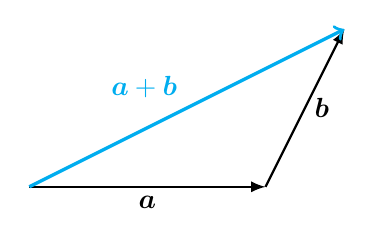
\begin{tikzpicture}
    \draw [-latex,thick] (3,0)--(4,2);
    \node [right] at ($(3,0)!0.5!(4,2)$) {$\bm{b}$};
    \draw [-latex,thick] (0,0)--(3,0);
    \node [below] at ($(0,0)!0.5!(3,0)$) {$\bm{a}$};
    \draw [->,very thick,cyan] (0,0)--(4,2);
    \node [above left,cyan] at ($(0,0)!0.5!(4,2)$) {$\bm{a}+\bm{b}$};
  \end{tikzpicture}
  \caption{三角形を作る方法}
  \label{fig: triangle}
\end{minipage}
\begin{minipage}[b]{0.3\columnwidth}
  \centering
  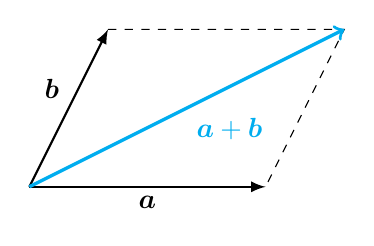
\begin{tikzpicture}
    \draw [-latex,thick] (0,0)--(1,2);
    \node [above left] at ($(0,0)!0.5!(1,2)$) {$\bm{b}$};
    \draw [-latex,thick] (0,0)--(3,0);
    \node [below] at ($(0,0)!0.5!(3,0)$) {$\bm{a}$};
    \draw [dashed] (1,2)--(4,2)--(3,0);
    \draw [->,very thick,cyan] (0,0)--(4,2);
    \node [below right,cyan] at ($(0,0)!0.5!(4,2)$) {$\bm{a}+\bm{b}$};
  \end{tikzpicture}
  \caption{平行四辺形を作る方法}
  \label{fig: parallelogram}
\end{minipage}
\end{figure}

\subsection{単位ベクトル}
\label{sec: vec-unit}

ユークリッド空間(実数を$n$個並べた全体の集合)において,3つの直交座標をそれぞれ$x$軸,$y$軸,$z$軸とする.
そのなかで\textbf{大きさを「1」に仕立てた}ベクトルを単位ベクトルという.
(単位○○は基本的に,○○の大きさを「1」に仕立てたもののことである.)

また,$x$軸と平行な単位ベクトルを$\bm{i}$,$y$軸と平行な単位ベクトルを$\bm{j}$,$z$軸と平行な単位ベクトルを$\bm{k}$とする.

\subsection{ベクトルの成分表示}

単位ベクトルと係数倍を用いて,一般にベクトルを次のような式で表せる.

\begin{equation}
  \bm{a}=A \bm{i}+B \bm{j}+C \bm{k}
\end{equation}

また,係数を座標のように表して,

\begin{equation}
  \bm{a}=(A \quad B \quad C)
\end{equation}

とも表せる.

\clearpage

\pagestyle{fancy}
\lhead{}
\rhead{\textbf{\thepage}}

\bibliographystyle{plain}
\bibliography{ref.bib}
\nocite{*}

\printindex

\end{document}